\let\lesson\undefined
\newcommand{\lesson}{\phantomlesson{Bài 9: Chuyển động ném}}
\chapter[Chuyển động ném ngang]{Chuyển động ném ngang}
\setcounter{section}{0}
\section{Lý thuyết}
\subsection{Khái niệm chuyển động ném ngang}
Chuyển động ném ngang là chuyển động có vận tốc ban đầu theo phương nằm ngang và chuyển động dưới tác dụng của trọng lực.
\subsection{Thí nghiệm}
Đồng thời thả viên bi B rơi tự do và ném viên bi A theo phương nằm ngang từ cùng một độ cao $h$. Hình \ref{fig:12.1} là ảnh chụp hoạt nghiệm tại nhiều thời điểm khác nhau khi thả hai viên bi
\begin{center}
	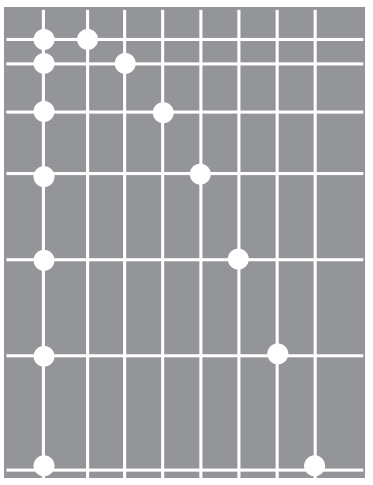
\includegraphics[width=0.2\linewidth]{../figs/VN10-2023-PH-TP012-1}
	\captionof{figure}{Ảnh chụp hoạt nghiệm chuyển động của hai viên bi A và B.}
	\label{fig:12.1}
\end{center}
Việc phân tích ảnh chụp hoạt nghiệm của thí nghiệm trên cho thấy rằng:\\
Tại bất kì thời điểm nào trong quá trình chuyển động, vị trí của viên bi A trên phương thẳng đứng cũng trùng với vị trí của bi B. Như vậy, thành phần chuyển động trên phương thẳng đứng của vật bị ném ngang là sự chuyển động rơi tự do.
\subsection{Phân tích kết quả thí nghiệm}
Từ kết quả thí nghiệm ở trên ta thấy rằng, chuyển động trên phương thẳng đứng của vật bị ném ngang là chuyển động rơi tự do và thành phần chuyển động trên phương nằm ngang của viên bi không ảnh hưởng đến thành phần chuyển động trên phương thẳng đứng của nó.\\
Ta có thể phân tích chuyển động ném ngang thành 2 thành phần chuyển động độc lập:
\begin{itemize}
	\item Thành phần chuyển động trên phương thẳng đứng.
	\item Thành phần chuyển động trên phương nằm ngang.
\end{itemize}
\begin{center}
\begin{tikzpicture}[scale=1, transform shape]  %horizontal projection
	%variable definitions
	\def\g{-9.8} %gravity
	\def\v{10} %velocity
	\def\ang{51} %angle
	\def\s{0.125}
	\pgfmathsetmacro{\c}{{(-1*(2/\g)*\v*sin(\ang))/2}}
	\pgfmathsetmacro{\a}{{(-1*(2/\g)*\v*sin(\ang))*.9}}
	
	\begin{axis}[
		width=.6\linewidth, %set bigger width
		height=3in,
		xmin={{\v*cos(\ang)*\c}},xmax=10, %{\v*cos(\ang)*\a+\s*\v*cos(\ang)}
		ymin=0,ymax={\v*\c*sin(\ang)+0.5*\g*(\c^2)},
		axis x line = top,
		every axis y label/.style={at={(axis description cs:0,-0.05)}},
		every axis x label/.style={at={(axis description cs:1.05,1)},anchor=west},
		xlabel=$x$,
		ylabel=$y$,
		axis y line = left,
		y axis line style={<-},
		x axis line style={<->},
		ticks = none,clip=false,
		]
		
		\tikzset{every mark/.append style={fill=red}}
		
		%flight path
		\addplot[
		dashed,
		domain={\v*cos(\ang)*\c}:10,
		samples=100,]
		{{\g*(x^2)/(2*\v^2*cos(\ang)^2)+x*tan(\ang)}};
		
		%vector at end
		\pgfmathsetmacro{\a}{{(-1*(2/\g)*\v*sin(\ang))*.9}}
		\coordinate (E) at (axis cs:{\v*cos(\ang)*\a},{\v*\a*sin(\ang)+0.5*\g*(\a^2)}){};
		\coordinate (F) at (axis cs:{\v*cos(\ang)*\a+\s*\v*cos(\ang))}, {\v*\a*sin(\ang)+0.5*\g*\a^2+\s*(\v*sin(\ang)+\g*\a)});
		\draw[thick,->](E)--(F);
		%			node[midway,sloped,above]{$\vec{V}$};
		\draw[densely dashed,thick,->](E)--(F |- E);
		%			node[midway,above]{$\vec{V}_x$};
		\draw[densely dashed,thick,->](E)--(F-| E);
		%			node[midway,left]{$\vec{V}_y$};
		
		\path plot[mark=*] coordinates {(E)};
		
		%vector at start
		\pgfmathsetmacro{\c}{{(-1*(2/\g)*\v*sin(\ang))/2}}
		\coordinate (L) at (axis cs:{\v*cos(\ang)*\c},{\v*\c*sin(\ang)+0.5*\g*(\c^2)});
		\coordinate (M) at (axis cs:{\v*cos(\ang)*\c+\s*\v*cos(\ang))},{\v*\c*sin(\ang)+0.5*\g*\c^2+\s*(\v*sin(\ang)+\g*\c)});
		\draw[thick,->](L)--(M)
		node[near end,sloped,above]{$\vec{v}_0$};
		
		\path plot[mark=*] coordinates {(L)};
		
		%vector 1/2 down
		\pgfmathsetmacro{\d}{{(-1*(2/\g)*\v*sin(\ang))*0.6}}
		\coordinate (P) at (axis cs:{\v*cos(\ang)*\d},{\v*\d*sin(\ang)+0.5*\g*(\d^2)});
		\coordinate (Q) at (axis cs:{(\v*cos(\ang)*\d+\s*\v*cos(\ang))},{\v*\d*sin(\ang)+0.5*\g*\d^2+\s*(\v*sin(\ang)+\g*\d)});
		\draw[thick,->](P)--(Q)
		%node[midway,sloped,above]{$\vec{V}$}
		;
		\draw[densely dashed,thick,->](P)--(Q|-P);
		%			node[midway,above]{$\vec{V}_x$};
		\draw[densely dashed,thick,->](P)--(Q-|P);
		%			node[midway,left]{$\vec{V}_y$};
		
		\path plot[mark=*] coordinates {(P)};
		
		%vector 3/4 down
		\pgfmathsetmacro{\f}{{(-1*(2/\g)*\v*sin(\ang))*0.7}}
		\coordinate (R) at (axis cs:{\v*cos(\ang)*\f},{\v*\f*sin(\ang)+0.5*\g*(\f^2)});
		\coordinate (S) at (axis cs:{(\v*cos(\ang)*\f+\s*\v*cos(\ang))},{\v*\f*sin(\ang)+0.5*\g*\f^2+\s*(\v*sin(\ang)+\g*\f)});
		\draw[thick,->](R)--(S);
		%			node[near end,above]{$\vec{v}$};
		\draw[densely dashed,thick,->](R)--(S|-R);
		%			node[near end,above,]{$\vec{v}_x$};
		\draw[densely dashed,thick,->](R)--(S-|R);
		%			node[near end,left]{$\vec{v}_y$};
		
		\path plot[mark=*] coordinates {(R)};
		
		%vector 1/4 down
		\pgfmathsetmacro{\e}{{(-1*(2/\g)*\v*sin(\ang))*0.8}}
		\coordinate (T) at (axis cs:{\v*cos(\ang)*\e},{\v*\e*sin(\ang)+0.5*\g*(\e^2)});
		\coordinate (U) at (axis cs:{(\v*cos(\ang)*\e+\s*\v*cos(\ang))},{\v*\e*sin(\ang)+0.5*\g*\e^2+\s*(\v*sin(\ang)+\g*\e)});
		\draw[thick,->,blue](T)--(U)
		node[near end,right=2mm]{$\vec{v}$};
		\draw[densely dashed,thick,->,blue](T)--(U|-T)
		node[near end,above]{$\vec{v}_x$};
		\draw[densely dashed,thick,->,blue](T)--(U-|T)
		node[near end,left]{$\vec{v}_y$};
		
		\path plot[mark=*] coordinates {(T)};
	\end{axis}
\end{tikzpicture}
	\captionof{figure}{Phân tích chuyển động ném ngang.}
\end{center}
\subsubsection{Tính chất của các chuyển động thành phần trên các trục}
\begin{itemize}
	\item Chuyển động thành phần theo trục O$x$ là chuyển động thẳng đều
	\begin{align*}
		a_x&=0,\\
		v_x&=v_0,\\
		x&=v_xt=v_0t.
	\end{align*}
	\item Chuyển động thành phần theo trục O$y$ là chuyển động rơi tự do không vận tốc đầu
	\begin{align*}
		a_y&=g,\\
		v_y&=0,\\
		y&=\dfrac{1}{2}gt^{2}.
	\end{align*}
\end{itemize}

%Biết hai chuyển động thành phần, ta suy ra được chuyển động của vật.
\subsubsection{Quỹ đạo của chuyển động ném ngang}
Phương trình quỹ đạo có thể suy ra bằng cách kết hợp hai phương trình chuyển động trên hai trục $x$ và $y$ 
\begin{equation*}
	y=\dfrac{g}{2v_0^2}x^2.
\end{equation*}
Quỹ đạo của vật ném ngang có dạng một nửa parabol, đỉnh tại vị trí ném.

\subsubsection{Thời gian chuyển động}
Thời gian chuyển động của vật ném ngang bằng thời gian rơi tự do của vật được thả từ cùng độ cao:
\begin{equation*}
	H=\dfrac{1}{2}gt^2\Rightarrow t=\sqrt{\dfrac{2H}{g}}.
\end{equation*}
Công thức trên cho thấy:
\begin{itemize}
	\item Thời gian rơi của vật bị ném ngang chỉ phụ thuộc độ cao $H$ của vật khi bị ném, không phụ thuộc vận tốc ném.
	\item Nếu từ cùng một độ cao, đồng thời ném ngang các vật khác nhau với các vận tốc khác nhau thì chúng đều rơi xuống đất cùng một lúc.
\end{itemize}
\subsubsection{Tầm ném xa}
\begin{center}
	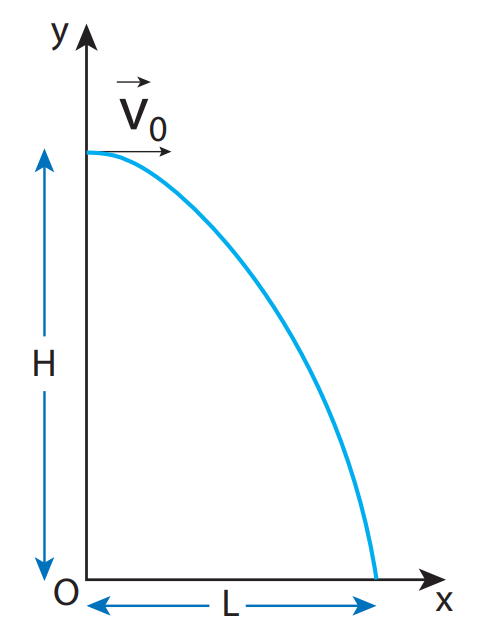
\includegraphics[width=0.2\linewidth]{../figs/VN10-2023-PH-TP012-3}
\end{center}
Là khoảng cách xa nhất vật đi được theo phương O$x$:
\begin{equation*}
	L = x_{\text{max}} = v_0 t = v_0 \sqrt{\dfrac{2H}{g}}.
\end{equation*}
Công thức trên cho thấy:
\begin{itemize}
	\item Tầm xa của vật bị ném ngang phụ thuộc vào độ cao $H$ của vật khi bị ném và vận tốc ném. Nếu từ cùng một độ cao đồng thời ném các vật khác nhau với vận tốc khác nhau thì vật nào có vận tốc ném lớn hơn sẽ có tầm xa lớn hơn.
	\item Nếu từ các độ cao khác nhau ném ngang các vật với cùng vận tốc thì vật nào được ném ở độ cao lớn hơn sẽ có tầm xa lớn hơn.
\end{itemize}
\subsubsection{Vận tốc của vật trong quá trình chuyển động}
Vận tốc của vật trong quá trình chuyển động là vận tốc tổng hợp của hai vận tốc thành phần $\overrightarrow{v_x}$  và $\overrightarrow{v_y}$
\begin{equation*}
	v=\sqrt{v^2_{\text{x}} + v^2_{\text{y}} } = \sqrt{v^2_0+ (gt)^2}.
\end{equation*}
Góc hợp bởi $\vec{v}$ và phương ngang
$$\tan\alpha=\dfrac{v_y}{v_x}$$
Tốc độ của vật khi chạm đất
\begin{equation*}
	v_\text{cđ}=\sqrt{v^2_{\text{x}} + v^2_{\text{y}} } = \sqrt{v^2_0+ \left(g\cdot\sqrt{\dfrac{2H}{g}}\right)^2}=\sqrt{v^2_0+2gH}.
\end{equation*}
\section{Mục tiêu bài học - Ví dụ minh họa}
\begin{dang}{Ghi nhớ đặc điểm và công thức \\ của chuyển động ném ngang}
	\viduii{1}{Một vật được ném ngang từ độ cao $h$ so với mặt đất ở nơi có gia tốc rơi tự do $g$. Thời gian chạm đất của vật là
		\begin{mcq}(2)
			\item $t=\sqrt{\dfrac{2h}{g}}.$
			\item $t=\dfrac{2h}{g}.$
			\item $t=\dfrac{h}{2g}$
			\item $t=\sqrt{\dfrac{h}{2g}}$
		\end{mcq}
	}
	{\hide{
		Thời gian chuyển động bằng thời gian rơi tự do của vật được thả từ cùng độ cao
		\begin{equation*}
			t=\sqrt{\dfrac{2h}{g}}.
		\end{equation*}
		
		\textbf{Đáp án: A}.
	}}

	\viduii{1}{Ở nơi có gia tốc rơi tự do là $g$, từ độ cao $h$ so với mặt đất, một vật được ném ngang với tốc độ ban đầu $v$. Tầm bay xa của vật là
		\begin{mcq}(2)
			\item $L = v_0 \sqrt{\dfrac{h}{2g}}.$
			\item $L = v_0 \dfrac{2h}{g}.$
			\item $L = v_0 \dfrac{h}{2g}.$
			\item $L = v_0 \sqrt{\dfrac{2h}{g}}.$ 
		\end{mcq}
	}
	{\hide{
		Tầm ném xa
		
		\begin{equation*}
			L = x_{\text{max}} = v_0 t = v_0 \sqrt{\dfrac{2h}{g}}.
		\end{equation*}
		
		\textbf{Đáp án: D}.
	}}
\end{dang}
\begin{dang}{Xây dựng phương trình quỹ đạo, \\giải bài toán về chuyển động ném ngang}
	\viduii{3}{Một viên đạn được bắn theo phương ngang ở độ cao $\SI{180}{m}$ phải có vận tốc ban đầu là bao nhiêu để ngay lúc chạm đất có $v = \SI{100}{m/s}$. Tính tầm ném xa của vật khi chạm đất.
	}
	{\hide{
		Thời gian chuyển động
		\begin{equation*}
			t=\sqrt{\dfrac{2h}{g}} = \SI{6}{s}
		\end{equation*}
		Vận tốc ban đầu 
		\begin{equation*}
			v^2 = v^2_{\text{x}} + v^2_{\text{y}}  = v^2_0+ (gt)^2 \Rightarrow v_0 =\sqrt{ v^2 -(gt)^2} = \SI{80}{m/s}.  
		\end{equation*}
		Tầm ném xa của vật khi chạm đất
		\begin{equation*}
			L=v_0 t  = \SI{480}{m}.
		\end{equation*}
		
	}}
	\viduii{3}{Từ sân thượng cao $\SI{20}{m}$ một người đã ném  một hòn sỏi theo phương ngang với $v_0 = \SI{4}{m/s}$, $g = \SI{10}{m/s^2}$.
		\begin{enumerate}[label=\alph*.]
			\item Viết phương trình chuyển động của hòn sỏi theo trục $Ox$, $Oy$.
			\item Viết phương trình quỹ đạo của hòn sỏi.
			\item Hòn sỏi đạt tầm xa bằng bao nhiêu? Tốc độ của nó khi vừa chạm đất.
		\end{enumerate}
	}
	{\hide{
		\begin{enumerate}[label=\alph*.]
			\item Chọn gốc tọa độ O ở sân thượng. Trục $Oy$ thẳng đứng hướng xuống, trục $Ox$ cùng hướng của vận tốc đầu. Gốc thời gian là lúc ném hòn sỏi. Phương trình chuyển động của hòn sỏi
			\begin{equation*}
				\begin{cases}
					x =v_0t = 4t. \\
					y = \dfrac{1}{2}gt^2 =5t^2.
				\end{cases}
			\end{equation*}
			\item Phương trình quỹ đạo của hòn sỏi thu được bằng cách kết hợp hai phương trình chuyển động thành phần trên hai trục
			\begin{align*}
				x&=v_0t	\quad\Rightarrow\quad t=\dfrac{x}{v_0}\\
				y&=\dfrac{1}{2}gt^{2}=\dfrac{1}{2}g\left(\dfrac{x}{v_0}\right)^{2}= \dfrac{5}{16}x^2.
			\end{align*}
			\item Khi rơi chạm đất $y = \SI{20}{\meter}$
			$$y=\dfrac{5}{16}x^2 =20 \quad\Rightarrow\quad x = \SI{8}{m}.$$
			
			Tầm xa của hòn sỏi $L =\SI{8}{m}.$
			
			Thời gian hòn sỏi chạm đất
			
			$$t=\sqrt{\dfrac{2h}{g}} = \SI{2}{s}.$$
			
			Tốc độ của hòn sỏi khi chạm đất 
			
			$$v=\sqrt{v^2_{\text{x}} + v^2_{\text{y}}} = \sqrt{v^2_0+ (gt)^2} = \SI{20,4}{m/s}.$$
		\end{enumerate}
	}}
\end{dang}